\documentclass{article}
\usepackage{tikz}
\usetikzlibrary{arrows,shapes,positioning,shadows,trees}


\tikzset{
every node/.style={draw,text width=2cm,drop shadow},
style1/.style= {rectangle, rounded corners=2pt, thin,align=center,fill=green!30},
style2/.style= {rectangle, rounded corners=6pt, thin,align=center,fill=green!60},
style3/.style= {rectangle,thin,align=left,fill=pink!60}
}

\begin{document}


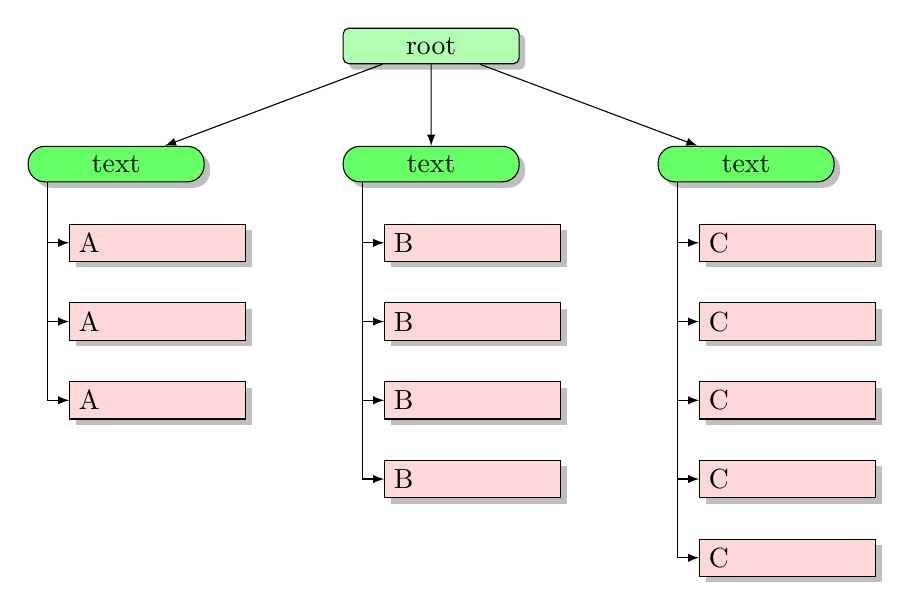
\begin{tikzpicture}[
remember picture,
level 1/.style={sibling distance=40mm},
edge from parent/.style={->,draw},
>=latex]

% the initial tree ("root" and "text nodes")
\node[style1] {root}
child {node[style2] (c1) {text}}
child {node[style2] (c2) {text}}
child {node[style2] (c3) {text}};

% the nodes below each of the "text" nodes
\node [style3,below of = c1,xshift=15pt] (c11) {A};
\node [style3,below of = c11] (c12) {A};
\node [style3,below of = c12] (c13) {A};

\node [style3,below of = c2,xshift=15pt] (c21) {B};
\node [style3,below of = c21] (c22) {B};
\node [style3,below of = c22] (c23) {B};
\node [style3,below of = c23] (c24) {B};

\node [style3,below of = c3,xshift=15pt] (c31) {C};
\node [style3,below of = c31] (c32) {C};
\node [style3,below of = c32] (c33) {C};
\node [style3,below of = c33] (c34) {C};
\node [style3,below of = c34] (c35) {C};

% lines from each "text" node to every one of its "children"
\foreach \value in {1,2,3}
  \draw[->] (c1.195) |- (c1\value.west);

\foreach \value in {1,...,4}
  \draw[->] (c2.195) |- (c2\value.west);

\foreach \value in {1,...,5}
  \draw[->] (c3.195) |- (c3\value.west);
\end{tikzpicture}

\end{document}

enter image description here